\documentclass[aspectratio=169]{beamer}

\usepackage{color}
\definecolor{airforceblue}{rgb}{0.36, 0.54, 0.66}
\definecolor{blue-green}{rgb}{0.0, 0.87, 0.87}
\definecolor{blue-violet}{rgb}{0.54, 0.17, 0.89}
\definecolor{cadet}{rgb}{0.33, 0.41, 0.47}
\definecolor{cordovan}{rgb}{0.54, 0.25, 0.27}

\mode<presentation>
{
    \usetheme{Madrid}
    \usefonttheme{professionalfonts} 
    \setbeamercolor{local structure}{fg=blue-green}
    \setbeamertemplate{itemize subitem}{\color{cordovan}$\blacktriangleright$}
}


\usepackage[utf8]{inputenc}
\usetheme{Madrid}
\usecolortheme{beaver}

\usepackage{caption}
\DeclareCaptionFormat{citation}{%
   \ifx\captioncitation\relax\relax\else
     \captioncitation\par
   \fi
   #1#2#3\par}
\newcommand*\setcaptioncitation[1]{\def\captioncitation{\textit{Source:}~#1}}
\let\captioncitation\relax
\captionsetup{format=citation,justification=centering}
\usepackage{mwe}% for example pictures
\usepackage{tikz,lmodern}
\usepackage[absolute,overlay,showboxes]{textpos}

\title{Comunicação em Datacenters}
\subtitle{Gerência de Redes}
\author[Leandro Silva, Luís Felipe] % (optional, for multiple authors)
{Leandro Souza da  Silva \\ Luís Felipe Mattos}
\institute{IC - Unicamp}


\date{ 06 de Dezembro de 2016 }
\logo{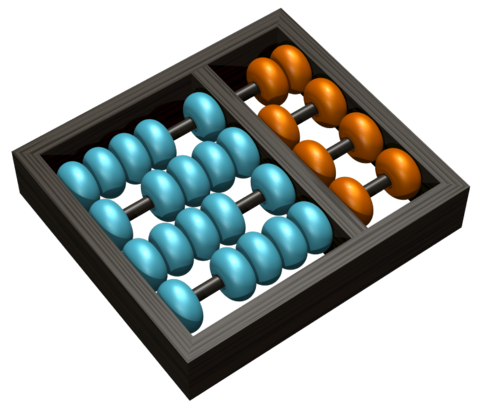
\includegraphics[height=1.0cm]{logo.png}}
 \newif\iflattersubsect
 


\AtBeginSection[] {
    \begin{frame}<beamer>
    \frametitle{Sumário} %
    \tableofcontents[currentsection]  
    \end{frame}
    \lattersubsectfalse
}

\AtBeginSubsection[] {
    \iflattersubsect
    \begin{frame}<beamer>
    \frametitle{Sumário} %
    \tableofcontents[currentsubsection]  
    \end{frame}
    \fi
    \lattersubsecttrue
}

 
\begin{document}

\begin{frame}
  \titlepage
\end{frame}

\begin{frame}{Sumário}
  \tableofcontents
  % You might wish to add the option [pausesections]
\end{frame}


\section{Introdução}

    \begin{frame} {Introdução}
        \centering
        \Large Visão Geral de um Data Center.
        \begin{figure}[ht]    
            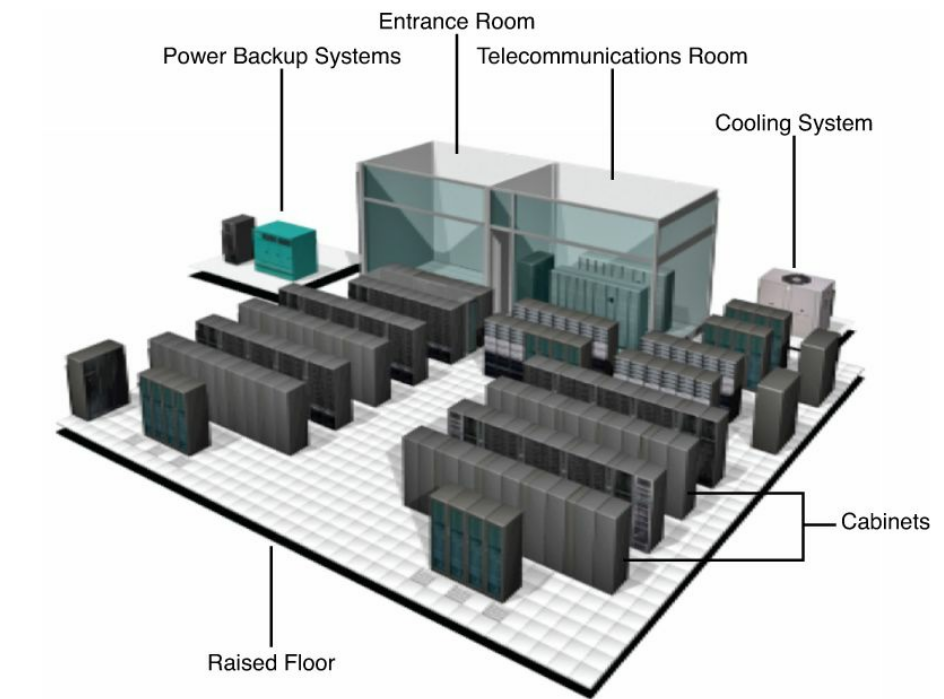
\includegraphics[scale=0.22]{datacenter.png}
            \caption{Data Center}
            \label{fig:data_center}
        \end{figure}

    \end{frame}
        
        
    \begin{frame} {Introdução}
        
         \begin{itemize}
         \setlength\itemsep{2em}
            \Large
            \item
                Com o crescimento da computação em nuvem, os datacenters passaram a receber funções novas.
                
             \item
                Certas aplicações necessitam de certos requisitos:
            \begin{itemize}
                \item
                    Escalabilidade
            
                \item
                    Tolerância a Falhas
                \item
                    Latêcia
                    
                 \item
                    Capacidade da Rede
                 \item
                    Virtualização               
            \end{itemize}
                    
         \end{itemize}
        
    \end{frame}


\section{Motivação} 

    \begin{frame} {Motivação}
            
        \centering
        \Large
             O consumo de dados pelos usuários está crescendo exponencialmente a cada ano.
            \begin{figure}[ht]    
                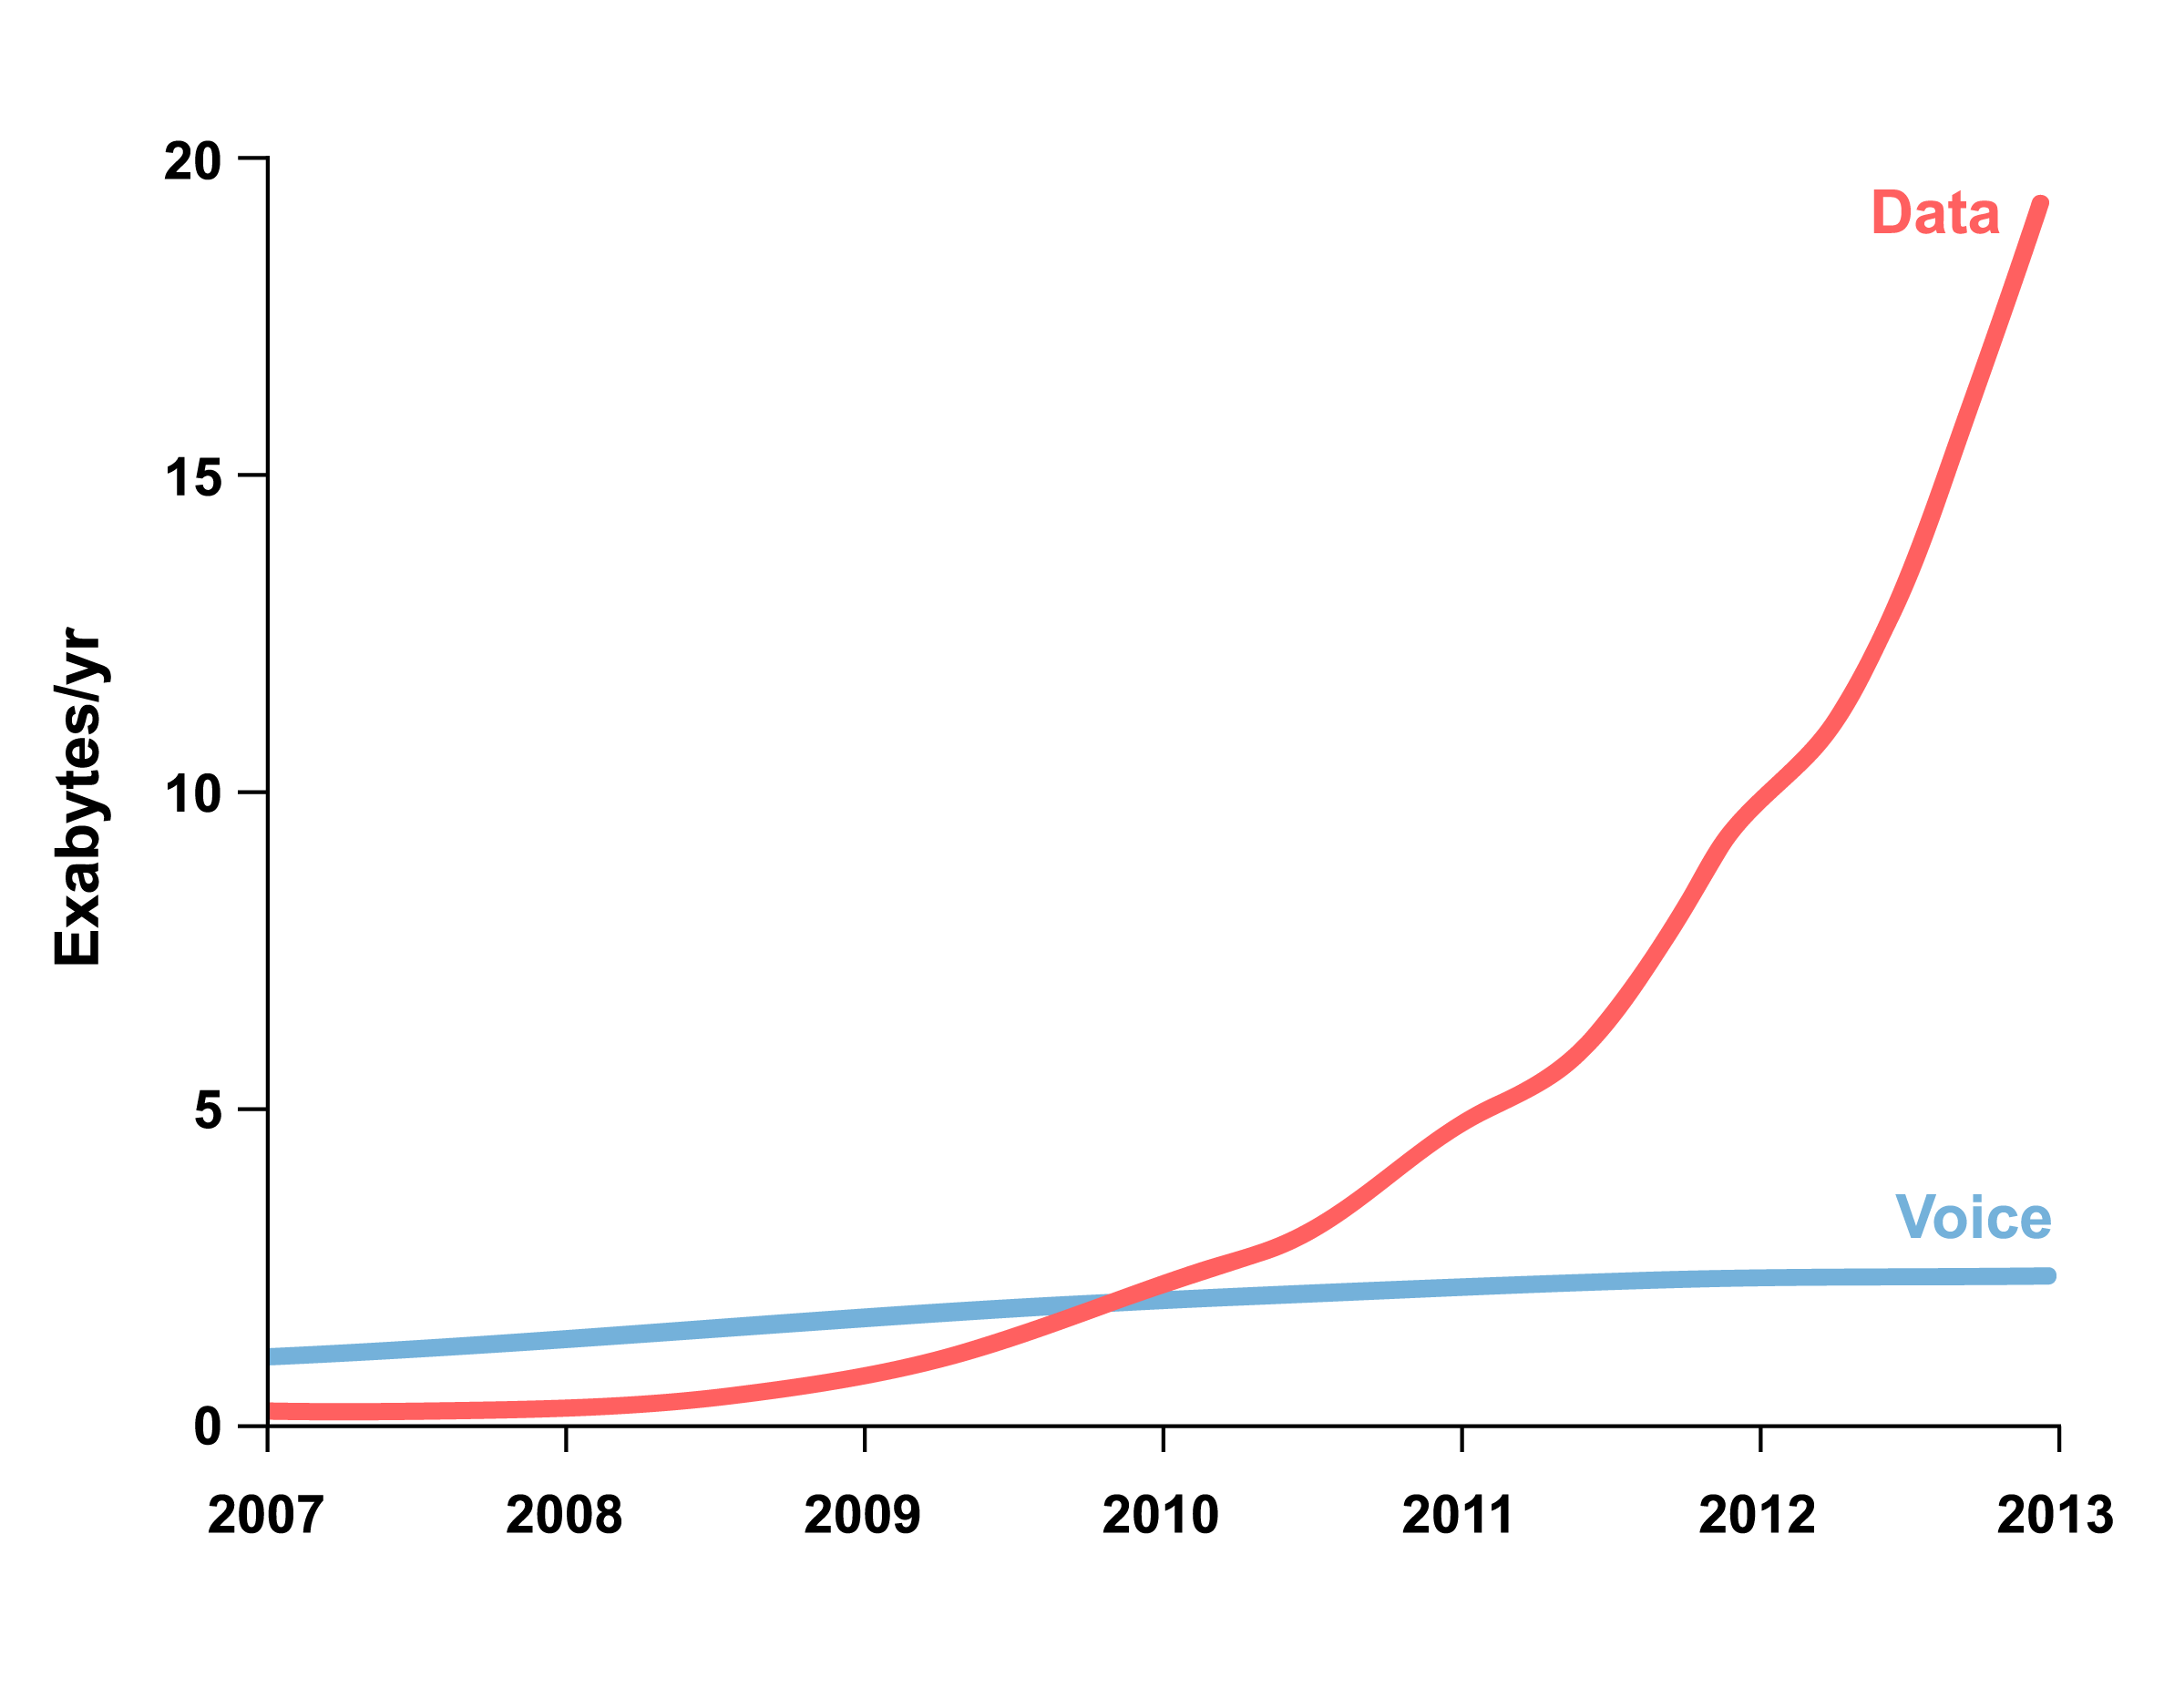
\includegraphics[scale=0.3]{consumo.png}
                \setcaptioncitation{The Cloud Begins With Coal , Ericsson Mobility Report, June 2013 }
                \caption{Consumo de dados e voz}
                \label{fig:consumo}
            \end{figure}

    \end{frame}
    
        \begin{frame} {Motivação}
            
            \centering
            \normalsize  
                Por causa disso, o número de servidores em Data Centers deve crescer exponencialmente para acompanhar a demanda, o que traz dificuldades em desenvolver redes eficientes e de baixo custo.
            \begin{figure}[ht]
       
                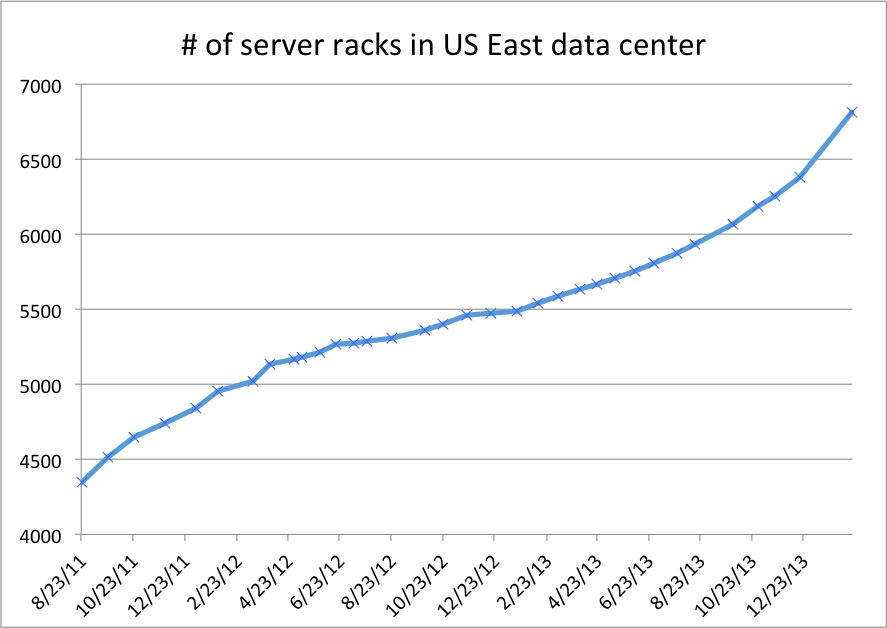
\includegraphics[scale=0.45]{servidores.png}
                \setcaptioncitation{  \href{https://huanliu.wordpress.com/category/cloud/}{https://huanliu.wordpress.com/category/cloud/ }}
                \caption{Número de servidores racks}
                \label{fig:servidores}
            \end{figure}
        
        \end{frame}
        
        \begin{frame} {Motivação}
                
            \Large
            Disponibilidade de dados e segurança se tornaram aplicações críticas.
            
        \end{frame}
                
            
        \begin{frame} {Motivação}
            \centering  
            \Large
            Por outro lado, a criação de novas tecnologias faz com que o custo dos componentes seja cada vez menor.
            \begin{figure}[ht]    
                            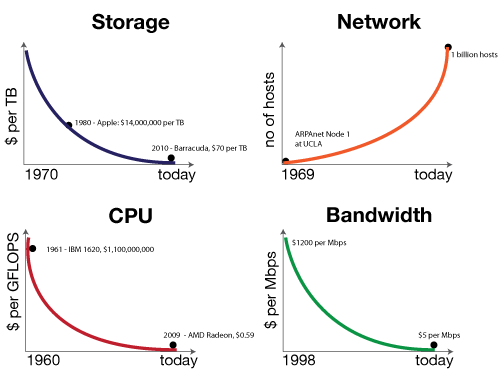
\includegraphics[scale=0.35]{custo.png}
                            \setcaptioncitation{  \href{http://radar.oreilly.com/2011/08/building-data-startups.html}{http://radar.oreilly.com/2011/08/building-data-startups.html }}
                            \caption{Custo de tecnologias}
                            \label{fig:custo}
                        \end{figure}
        \end{frame} 
            
        \begin{frame} {Motivação}
            \centering
            \Large
            Apesar disso, surge uma dificuldade cada vez maior de criar redes escaláveis exponencialmente sem que haja perda de eficiência.
            \begin{figure}[ht]    
                            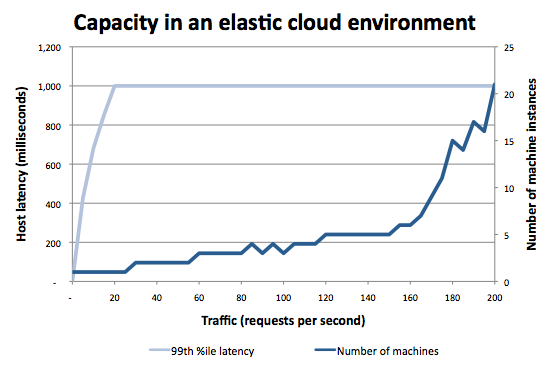
\includegraphics[scale=0.35]{capacity.png}
                             \setcaptioncitation{  \href{http://www.bitcurrent.com/the-clouds-most-important-equation/}{http://www.bitcurrent.com/the-clouds-most-important-equation/}}
                             %\href{http://tex.stackexchange.com/q/20800/5701}{\beamergotobutton{Link}}
                             \caption{Capacidade elástica em ambiente de nuvem}
                    
                            \label{fig:capacity}
                        \end{figure}
        \end{frame} 
            
        
\section{Topologias} 
    
    \subsection{Tradicionais}
    
        \begin{frame} {Topologias Tradicionais}
           \begin{columns}    
             \column{0.4\textwidth}  
             \begin{itemize}
              
             \setlength\itemsep{2em}
                \Large
                \item
                    Baseadas em ávrores.
                    
              
                \begin{itemize}
                    
                    \item
                        Basic Tree
                
                    \item
                        Fat-Tree
                
                     \item
                        VL2 
                                
                \end{itemize}
                        
             \end{itemize}
                
              \begin{itemize}
               
              \setlength\itemsep{2em}
                 \Large
                 \item
                     Recursivas.
                     
               
                 \begin{itemize}
                    
                     \item
                         Dcell
                 
                     \item
                         Bcube
                 
                      \item
                         FiConn
                                 
                       \item
                        FlatNet
                       
                       \item
                        SprintNet
                 \end{itemize}
                         
              \end{itemize}
          \end{columns} 
         \end{frame}
    
     \begin{frame} {Basic Tree}
            \begin{figure}[ht]    
                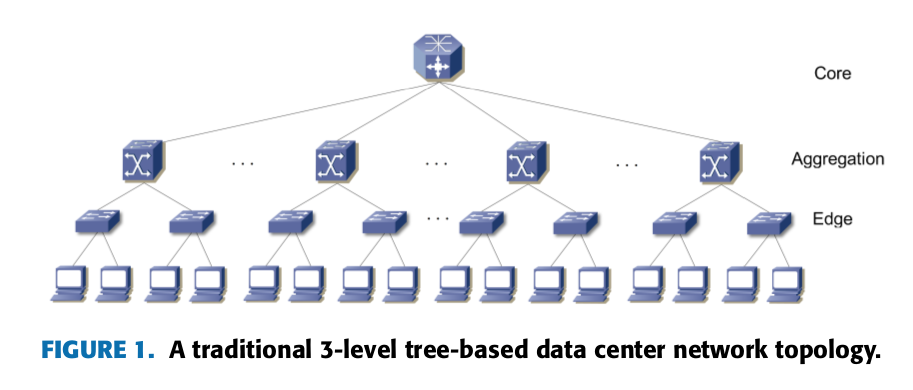
\includegraphics[scale=0.38]{basic_tree.png}
                
               
                \label{fig:consumo}
            \end{figure}

     
     \end{frame}
     
     
      \begin{frame} {Fat Tree, baseada na rede CLOS}
             \begin{figure}[ht]    
                 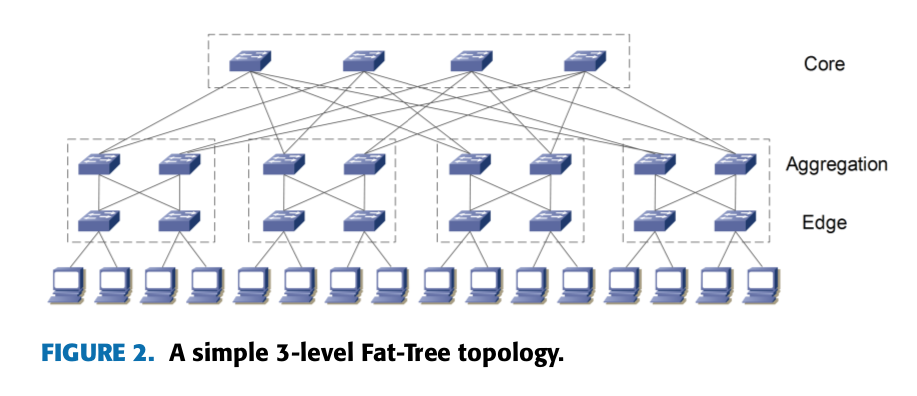
\includegraphics[scale=0.38]{fat_tree.png}
                 
                
                 \label{fig:consumo}
             \end{figure}
 
      
      \end{frame}
      
       \begin{frame} {VL2}


         \begin{itemize}
             \Large
             \item
                 Switches em uma topologia de rede CLOS
         
             \item
                 Usa o VLB (Valiant Load Balancing) para distribuir tráfego entre os caminhos da rede
         
              \item
                 Usa o protocolo ARP (Address Resolution Protocol) para que seja escalável para um número grande de servidores
                         
              
         \end{itemize}
  
       
       \end{frame}
    
    	\begin{frame} {Topologias Tradicionais}
			Topologias recursivas
		\end{frame}

		\begin{frame} {Topologias Recursivas: Dcell}
			Baseada em células interligadas entre servidores
			\begin{figure}[ht]    
				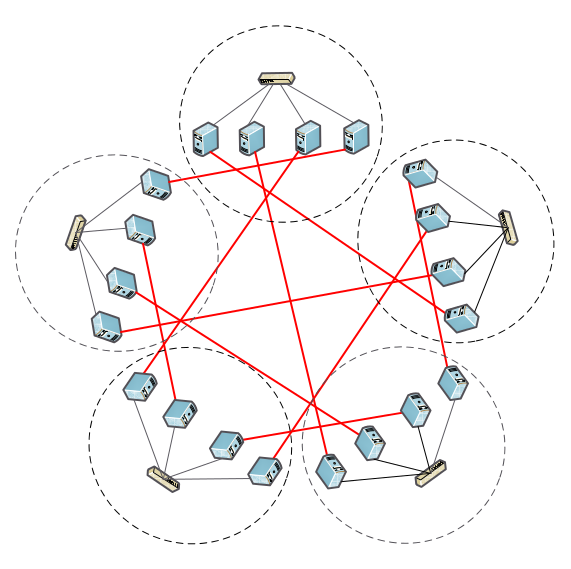
\includegraphics[scale=0.3]{imagens/dcell.png}
				\label{fig:sample_figure}
			\end{figure}
		\end{frame}

		\begin{frame} {Topologias Recursivas: Bcube}
			Baseada em células interligadas entre switches
			\begin{figure}[ht]    
				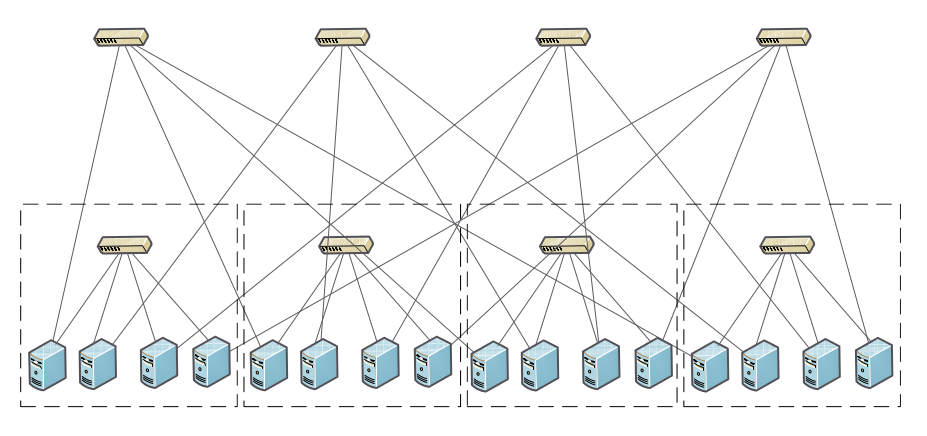
\includegraphics[scale=0.3]{imagens/bcube.png}
				\label{fig:sample_figure}
			\end{figure}
		\end{frame}

		\begin{frame} {Topologias Recursivas: FiConn}
			Semelhante à Dcell, mas o grau de cada célula é sempre 2
			\begin{figure}[ht]    
				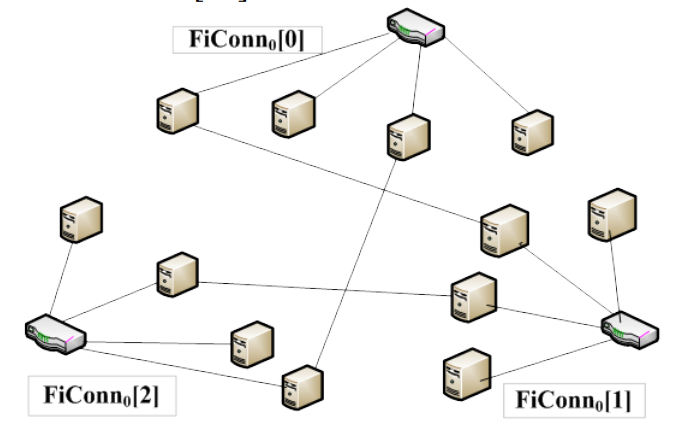
\includegraphics[scale=0.3]{imagens/ficonn.png}
				\label{fig:sample_figure}
			\end{figure}
		\end{frame}

		\begin{frame} {Topologias Recursivas: FlatNet}
			Semelhante ao BCube, porém é mais escalável
			\begin{figure}[ht]    
				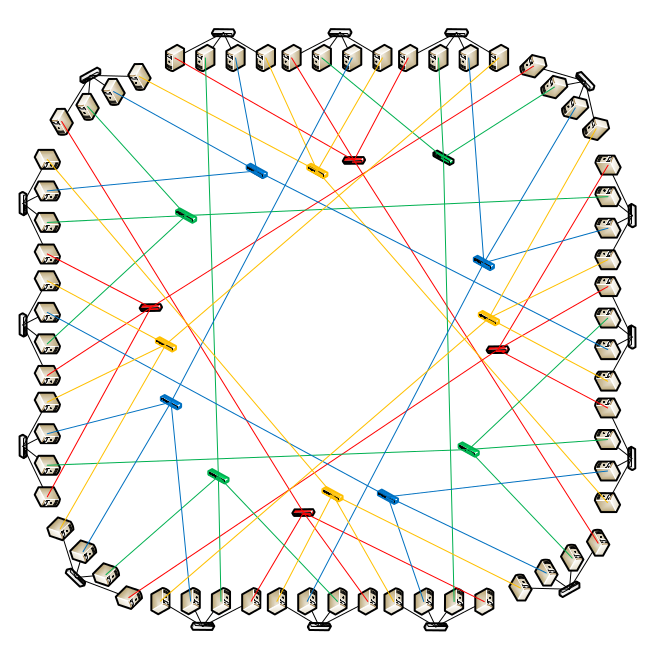
\includegraphics[scale=0.3]{imagens/flatnet.png}
				\label{fig:sample_figure}
			\end{figure}
		\end{frame}

		\begin{frame} {Topologias Recursivas: SprintNet}
			Semelhante à DCell, porém as células são compostas por 4 servidores e 2 switches de 6 portas
			\begin{figure}[ht]    
				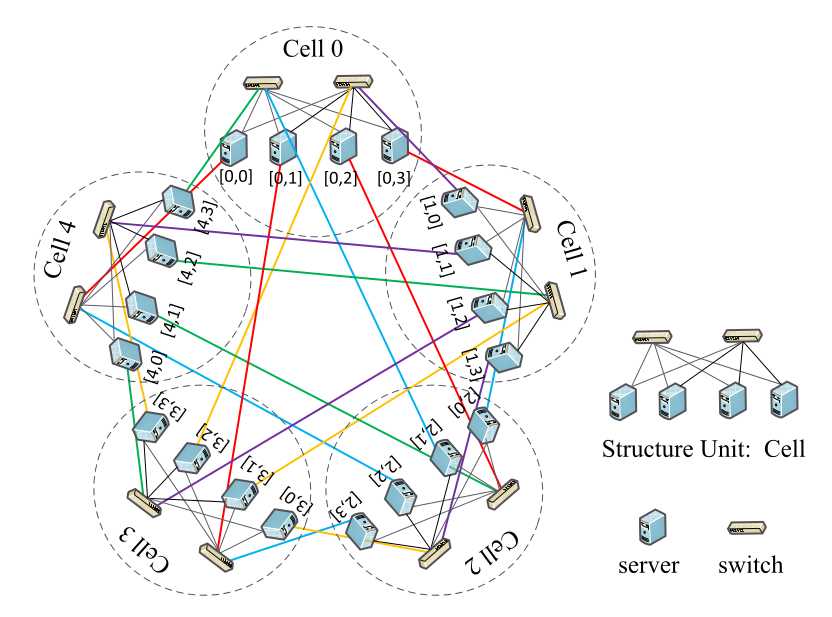
\includegraphics[scale=0.3]{imagens/springnet.png}
				\label{fig:sample_figure}
			\end{figure}
		\end{frame}

		\begin{frame} {Comparação}
			\begin{figure}[ht]   
				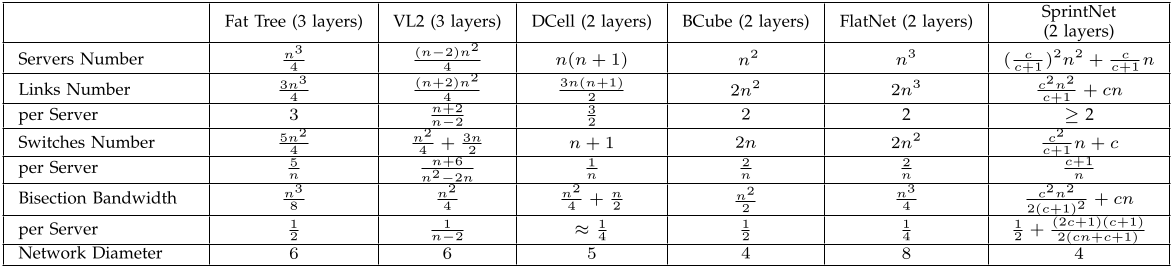
\includegraphics[scale=0.35]{imagens/tabela.png}
				\label{fig:sample_figure}
			\end{figure}
		\end{frame}

		\subsection{SDN}
		
		\begin{frame} {SDN em Datacenters}
			Com o avanço do SDN, a ideia mais básica é definir servidores virtualizados e criar uma rede virtualizada
			\begin{figure}[ht]   
				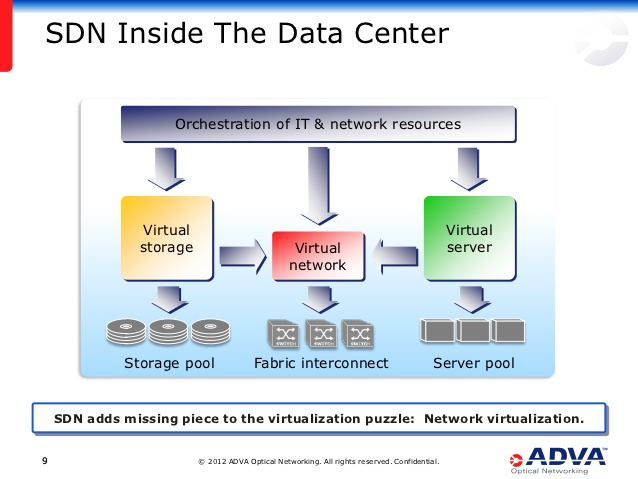
\includegraphics[scale=0.35]{imagens/inside-sdn.jpg}
				\label{fig:sample_figure}
			\end{figure}
		\end{frame}

		\begin{frame} {SDN em Datacenters}
			Esta técnica já é utilizada atualmente (PayPal por exemplo)
			\begin{figure}[ht]   
				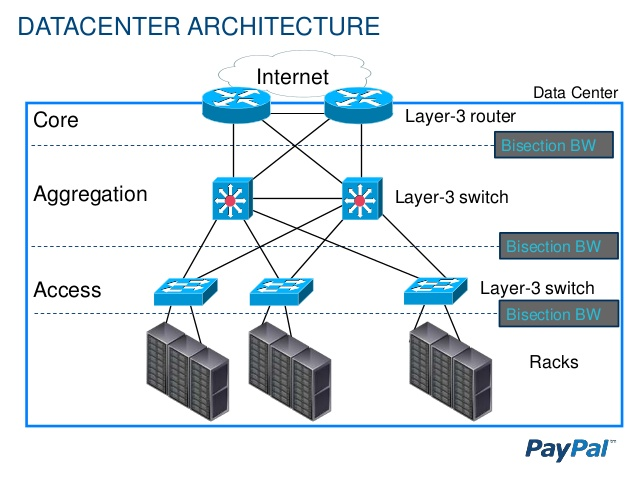
\includegraphics[scale=0.3]{imagens/sdn-1.jpg}
				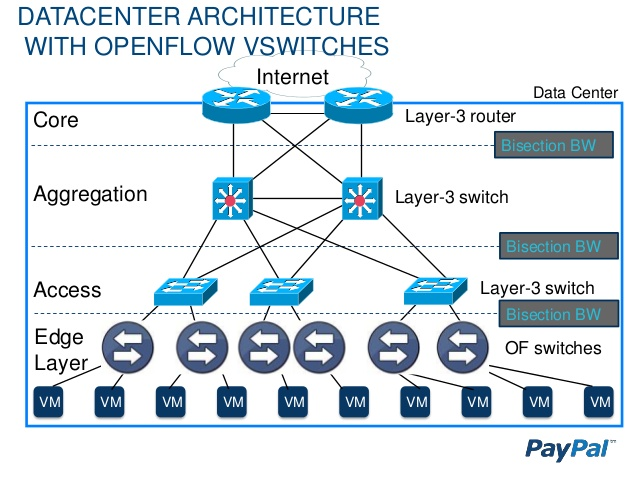
\includegraphics[scale=0.3]{imagens/sdn-2.jpg}
				\label{fig:sample_figure}
			\end{figure}
		\end{frame}

		\begin{frame} {SDN em Datacenters}
			\begin{figure}[ht]   
				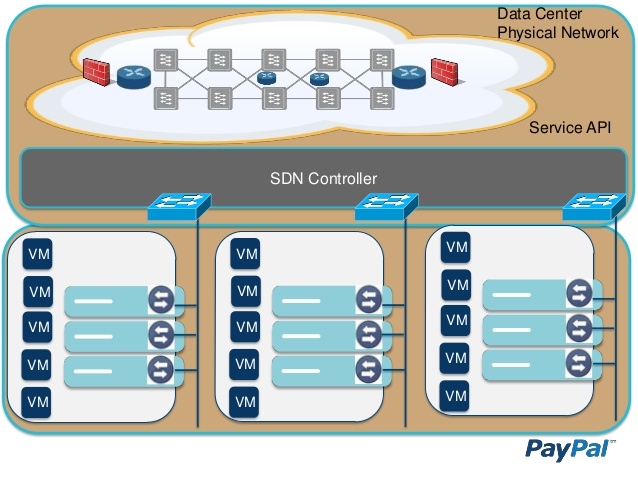
\includegraphics[scale=0.4]{imagens/sdn-3.jpg}
				\label{fig:sample_figure}
			\end{figure}
		\end{frame}


\section{Protocolos}
    \subsection{Roteamento}
    
    
    \begin{frame}{Protocolos}
    \huge
    Datacenters têm alguns requisitos básicos,  mas que causam algumas dificuldades:
   
      \begin{columns}    
        \column{0.5\textwidth}   
          \begin{itemize}
              \large            
              \item
                  RTTs precisam ser da ordem de microsegundos
          
              \item
                  Poucas multiplexações
          
               \item
                  Perda de pacotes baixa
                \item
                    Lidar com Incast
                    
               
                          
          \end{itemize}
     \column{0.5\textwidth}   
     \begin{figure}[ht]    
                     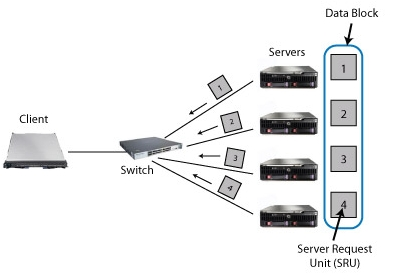
\includegraphics[scale=0.3]{problems.jpg}
                     
                    
                     \label{fig:problems}
                 \end{figure}
    
    
    \end{columns}
    
     
    
    \end{frame}
    
 
    \begin{frame} {Roteamento}
      				
                  \begin{columns}[t]    
                  	
                    \column{0.3\textwidth}  
                    
                    \begin{itemize}
                     
                    \setlength\itemsep{2em}
                       \large
                       \item
                          Esquemas para TE
                           
                       \begin{itemize}
                           
                           \item
                              	ECMP
                       
                           \item
                              	VL2
                       
                            \item
                               DARD 
                                       
                       \end{itemize}
                               
                    \end{itemize}
                   
                      
                 \end{columns} 
                
    \end{frame}
       

 
    \begin{frame} {ECMP}
      				
   
	  Falar do ECMP
	        
                
    \end{frame}     
    
    
    
 
    \begin{frame} {VL2}
      				
   
	  Falar do VL2
	        
                
    \end{frame}     
    
    
    
 
    \begin{frame} {DARD}
      				
   
	  Falar do DARD
	        
                
    \end{frame}     
    
    
    \subsection{Transporte}
	\begin{frame} {Transporte}
	      				
           \begin{columns}[t]    
                 	
             \column{0.3\textwidth}  
             
             \begin{itemize}
              
             \setlength\itemsep{2em}
                \large
                \item
                   Deadline-Agnostic
                    
                \begin{itemize}
                    
                    \item
                          DCTCP
                
                    \item
                           MPTCP
                
                     \item
                        ICTCP 
                                
                \end{itemize}
                        
             \end{itemize}
              
         
             
             \begin{itemize}
              
             \setlength\itemsep{2em}
                \large
                \item
                   Deadline-Aware
                    
                \begin{itemize}
                    
                    \item
                          $D^3$
                
                    \item
                            $D^2$TCP
                
                     \item
                        DeTail 
                        
                       \item
                        PDQ 
                                
                \end{itemize}
                        
             \end{itemize}
          \end{columns} 
         
	    \end{frame}
	       
	
	 
            
    \begin{frame} {DCTCP}
      				
   
	  Falar do DCTCP
	        
                
    \end{frame}     
    
    
    
 
    \begin{frame} {MPTCP}
      				
   
	  Falar do MPTCP
	        
                
    \end{frame}     
    
    
    
 
    \begin{frame} {ICTCP}
      				
   
	  Falar do ICTCP
	        
                
    \end{frame}  
    
    
  
    \begin{frame} {Deadline-Aware: $D^3$}
		\begin{itemize}
		 	\item
		 		Recebe a informação do tamanho do fluxo e o deadline
		 	\item
				Algoritmo guloso para tentar cumprir o máximo de deadlines possíveis
		 	\item
				Roteadores tentam alocar uma taxa adequada para cada fluxo
		 	\item
				Emissor envia dados com a mínima taxa alocada no próximo RTT
		 	\item
				A fonte periodicamente requisita uma nova taxa baseada no deadline e o tamanho do fluxo restante
		 \end{itemize}
	\end{frame}

	\begin{frame} {Deadline-Aware: $D^3$}
		\begin{itemize}
		 	\item
		 		Switches precisam de modificações para lidar com as requisições
		 	\item
				Não é compatível com o TCP tradicional, por causa da alocação de largura banda baseado em prioridades sem a informação do deadline no header
		 	\item
				Alocação com algoritmo guloso pode alocar largura de banda para fluxos com deadlines distantes ao invés de deadlines próximos, o que pode causar maior perda de deadlines
		 	\item
				Requisições constantes de taxas tem um overhead
		 \end{itemize}
	\end{frame}

	\begin{frame} {Deadline-Aware: $D^2TCP$}
		\begin{itemize}
		 	\item
		 		Baseado no DCTCP, mas leva o deadline em consideração para redimensionar a janela de congestionamento
		 	\item
				Se a maioria dos deadlines são próximos, ainda pode ocorrer congestionamento
		 	\item
				Se a maioria dos deadlines são distantes, ocorrerá a sub-utilização da rede e baixa taxa de transferência
		 	\item
				Se todos os deadlines são próximos, estão competindo pela largura de banda e nenhum fluxo é adiado, todos os deadlines não serão cumpridos. Caso um fluxo seja adiado, todos os outros podem ser cumpridos.
		 	\item
				O problema é saber qual fluxo sacrificar para satisfazer o máximo de deadlines possíveis
		 \end{itemize}
	\end{frame}

	\begin{frame} {Deadline-Aware: $DeTail$}
		\begin{itemize}
		 	\item
		 		Fluxos são associados com prioridades e os switches usam filas de prioridades nas portas de saída e de entrada
		 	\item
				Cada camada da abstração da rede tem uma função
		 \end{itemize}

		\begin{figure}[ht]   
			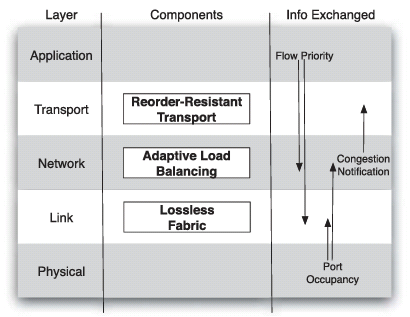
\includegraphics[scale=0.5]{imagens/detail.png}
			\label{fig:sample_figure}
		\end{figure}
	\end{frame}

	\begin{frame} {Deadline-Aware: $DeTail$}
		Enlace:
		\begin{itemize}
		 	\item
		 		Controle de fluxo “hop-by-hop” 
		 	\item
				Tenta amenizar o bloqueio de “head-of-line” (HOL)
		 	\item
				Recebe informações da camada de rede em relação ao balanco de carga adaptativo
		 	\item
				Recebe informações da camada de transporte sobre o estado do ECN
		 \end{itemize}
	\end{frame}

	\begin{frame} {Deadline-Aware: $DeTail$}
		Rede:
		\begin{itemize}
		 	\item
		 		Balanço de carga adaptativo baseado em pacotes de acordo com o nível de congestionamento
		 	\item
				Pode transmitir pacotes por caminhos que estão com pouca carga
		 \end{itemize}
	\end{frame}

	\begin{frame} {Deadline-Aware: $DeTail$}
		Rede:
		\begin{itemize}
		 	\item
		 		Usa o ECN para marcar fluxos de baixa prioridade quando os bytes transmitidos para o destino ultrapassam um certo limiar
		 	\item
				Previne congestionamento persistente
		 \end{itemize}
	\end{frame}

	\begin{frame} {Deadline-Aware: $DeTail$}
		Aplicação:
		\begin{itemize}
		 	\item
		 		Seleciona as prioridades de cada fluxo baseado na sensibilidade de latência
		 \end{itemize}
	\end{frame}

	\begin{frame} {Deadline-Aware: $PDQ$}
		\begin{itemize}
		 	\item
		 		Semelhante ao $D^3$, mas ao contrário do $D^3$, escalona taxas de acordo com a criticalidade dos fluxos ao invés da política “first-come first-serve”
		 	\item
		 		Duas políticas de alocação, implementadas de forma totalmente distribuída:
				\begin{itemize}
				 	\item
				 		EDF (Earliest Deadline First)
				 	\item
						SJF (Shortest Job First)
				 \end{itemize}
		\end{itemize}
	\end{frame}


\section{Tendências}
    \begin{frame} {Facebook Fabric}
        
        
        
	  \begin{itemize}
		                        
		            \item
		                  A próxima geração de data center do Facebook
		     
		        
		             \item
		               Topologia não hierarquizada
		                
		               \item
		                 Rede de alto desempenho
		               \item
		               		Sem oversubscription
		               		                   
		     
		                
		     \end{itemize}
	        
   
              \begin{columns}    
                \column{0.5\textwidth}   
              \begin{figure}[ht]    
                  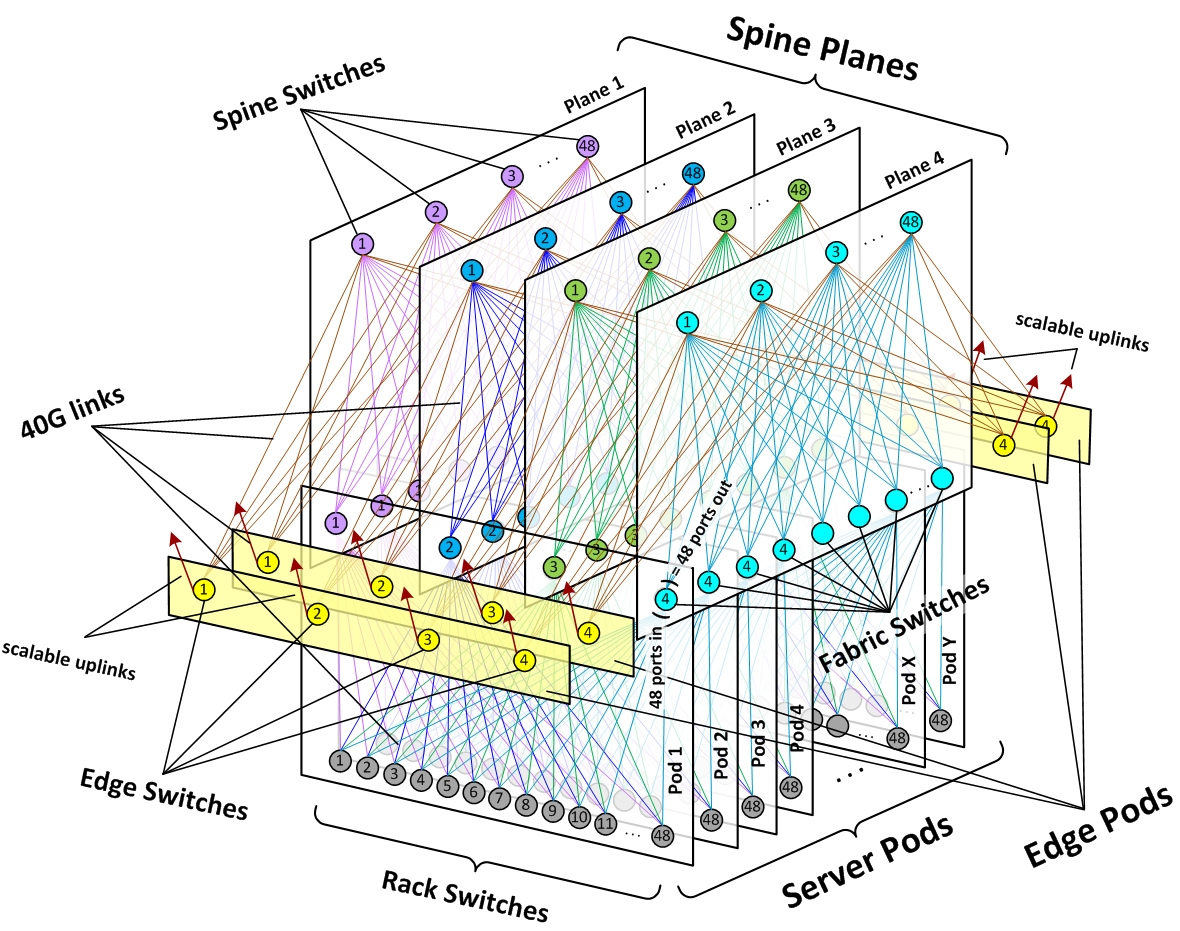
\includegraphics[scale=0.3]{scheme_fabric.jpg}
                    
                                            
                 
                 
                  \label{fig:problems}
              \end{figure}
                         
             \column{0.5\textwidth}   
             \begin{figure}[ht]    
                             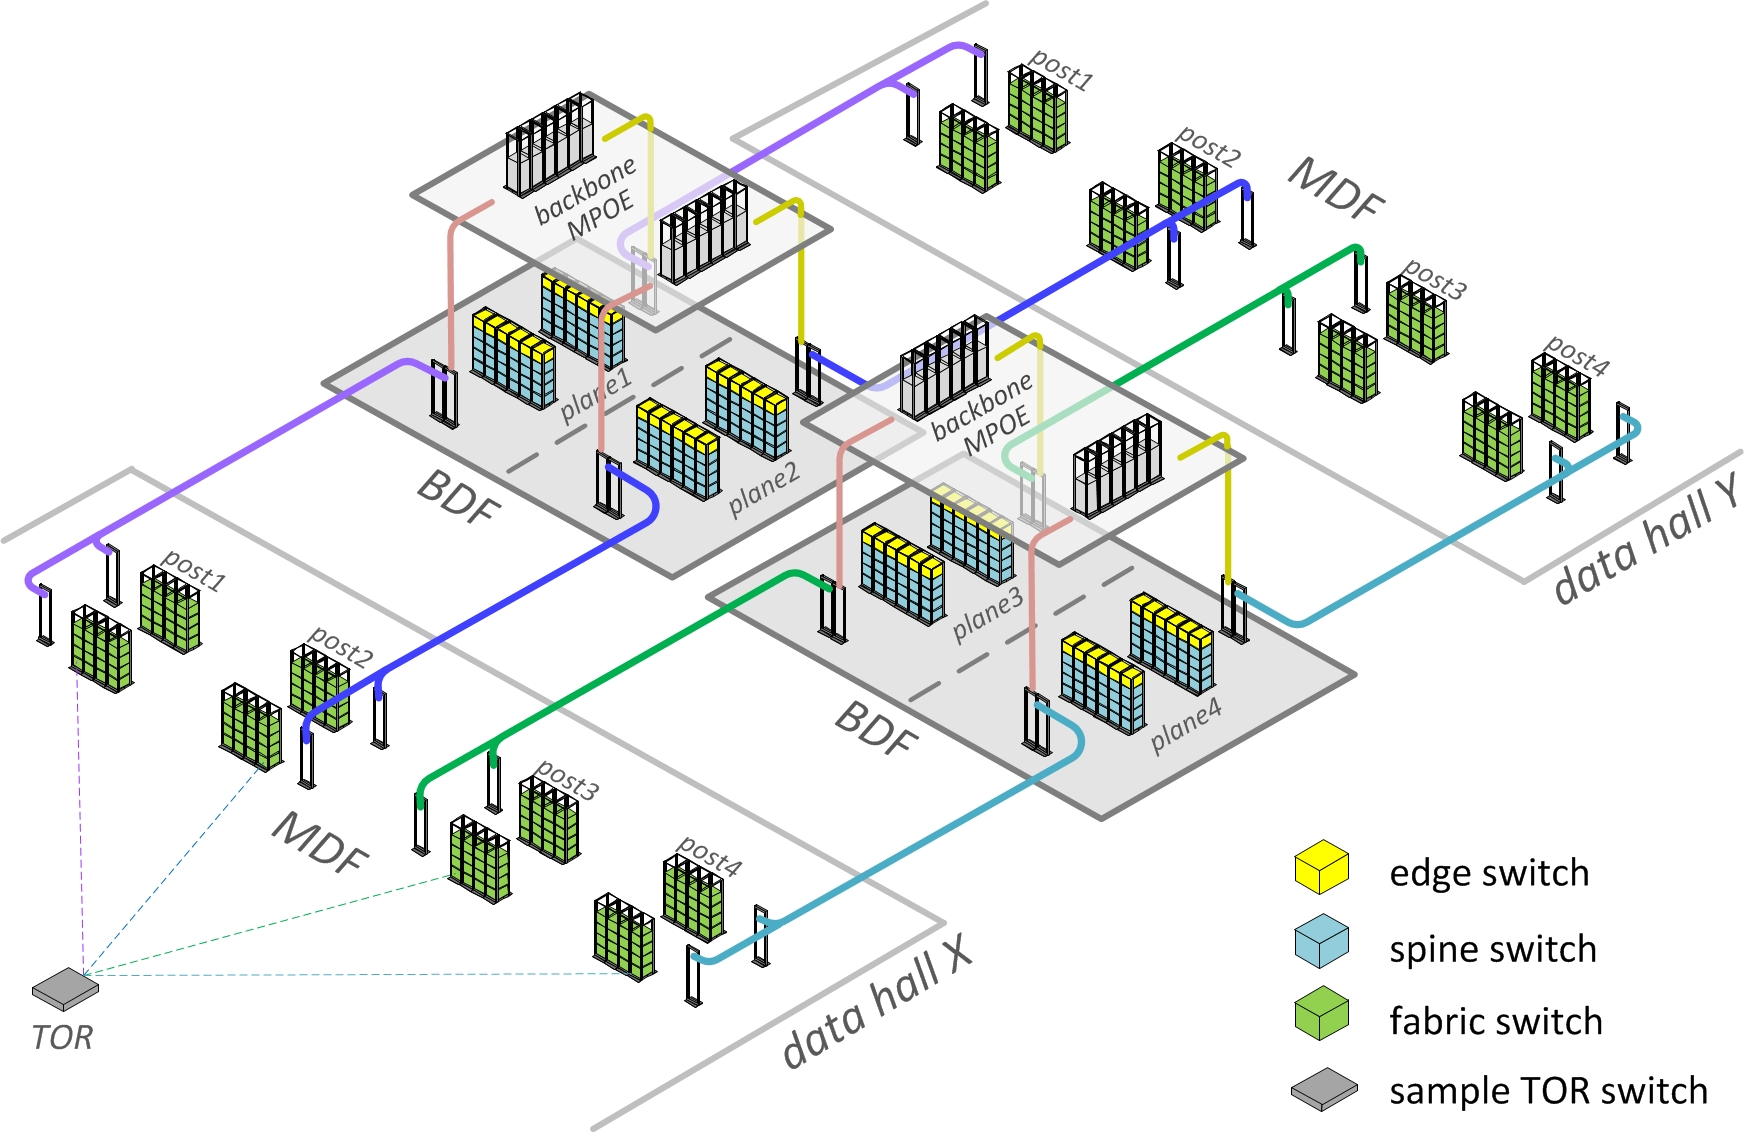
\includegraphics[scale=0.23]{phisic_fabric.jpg}
                          
                                                                     
                                           
                            
                             \label{fig:problems}
                         \end{figure}
            
            
            \end{columns}
            
             
          
    \end{frame}

\section{Conclusão}
    \begin{frame} 
        Ponha aqui seu texto
    \end{frame}
        
\section{Pergunta}
    \begin{frame} 
        Ponha aqui seu texto
    \end{frame}
    
\end{document}
